\documentclass[10pt,a4paper,english]{report}

\usepackage{fontspec}
\usepackage{xunicode}
\usepackage{babel}
\usepackage{graphicx}

\usepackage{amsthm}
\usepackage{amsmath}
\usepackage{amssymb}
\usepackage{mathrsfs}

\usepackage{geometry}
\geometry{top=2cm, bottom=2cm, left=2cm , right=2cm}

\usepackage{hyperref}

\usepackage{float}
\usepackage{diagbox}
\usepackage{minted}

\title{Git Tutorial}
\author{Nils Van Zuijlen}
\date{\today}

\setcounter{tocdepth}{3}

\begin{document}

\maketitle

\tableofcontents

\part{Basics}

\chapter{What is git?}

    Git is a distributed version control system for managing source code.

    Ok, so what is version control? Simply put, version control is a system for tracking changes to files. As you modify files, the version control system records and saves each change. This allows you to restore a previous version of your code at any time.

    Without a version control system, you are stuck manually saving multiple versions of your file using different dates and/or names (e.g. \verb|12-02-2016-monkey_code.php|; \verb|12-03-2016-monkey_code.php|). This method is time-consuming and impractical when you are dealing with hundreds of files.

    \begin{figure}[ht]
    \begin{center}
    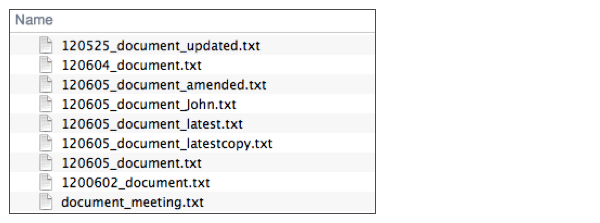
\includegraphics[scale=0.5]{images/what_is_git_001.png}
    \end{center}
    \caption{Examples of backing up a file}
    \end{figure}

    Fact: \emph{This type of versioning will only end in tears.}

    Renaming a file also doesn't give you any context as to what changes were made or who they were made by. When multiple team members edit the same file, overwriting may occur and it becomes difficult to keep up with the latest file version.

    With Git, you can easily follow your source code's revision history and track changes. You can also go back in time to learn about how the version has changed and who has made the changes. When the latest version of a file is on a shared repository, Git will prevent unintentional overwrites by anyone on your team who has an older version of the file.

    \begin{figure}[ht]
    \begin{center}
    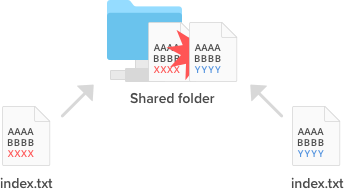
\includegraphics[scale=0.5]{images/what_is_git_002.png}
    \end{center}
    \caption{Failure examples while working as a team}
    \end{figure}

    \begin{figure}[ht]
    \begin{center}
    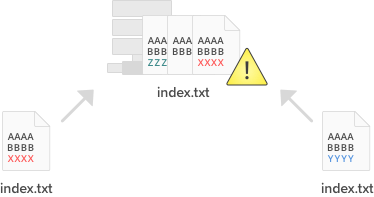
\includegraphics[scale=0.5]{images/what_is_git_003.png}
    \end{center}
    \caption{Examples of team works using the management of versions}
    \end{figure}

    A version control system like Git makes it easy to:
    \begin{itemize}
        \item Keep track of code history
        \item Collaborate on code as a team
        \item See who made which changes
        \item Deploy to staging or production
    \end{itemize}

\chapter{Git workflow}
    \label{chap:workflow}

    There are three main components of a Git project:
    \begin{itemize}
        \item Repository
        \item Working tree
        \item Index
    \end{itemize}

    The repository, or repo, is the “container” that tracks the changes to your project files. It holds all the commits -- a snapshot of all your files at a point in time -- that have been made. You can access the commit history with the Git log.

    The working tree, or working directory, consists of files that you are currently working on. You can think of a working tree as a file system where you can view and modify files.

    The index, or staging area, is where commits are prepared. The index compares the files in the working tree to the files in the repo. When you make a change in the working tree, the index marks the file as modified before it is committed.

    \begin{figure}[ht]
    \begin{center}
    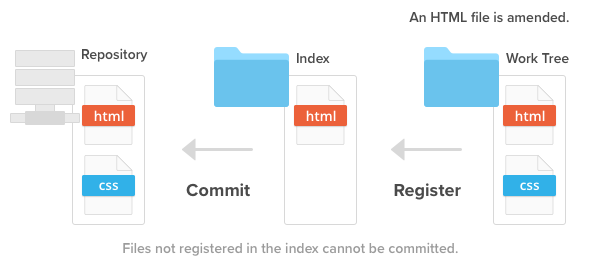
\includegraphics[scale=0.5]{images/git_workflow_001.png}
    \end{center}
    \caption{The three main components of a Git project: the repository, index, and working tree.}
    \end{figure}

    Below is the basic Git workflow:
    \begin{itemize}
        \item Modify files in the working tree.
        \item Stage the changes you want to be included in the next commit.
        \item Commit changes. Committing will take the files from the index and store them as a snapshot in the repository.
    \end{itemize}

    \section{Three states of Git files}

    As you can probably guess from the Git workflow, files can be in one of three states:
    \begin{itemize}
        \item Modified
        \item Staged
        \item Committed
    \end{itemize}

    When a file is first modified, the change can only be found in the working tree. You must stage the changes you want to be included in your next commit. The index contains all file changes that will be committed. Once you have finished staging files, commit them with a message describing what you changed. The modified files are now safely stored in the repo.

    \begin{figure}[ht]
    \begin{center}
    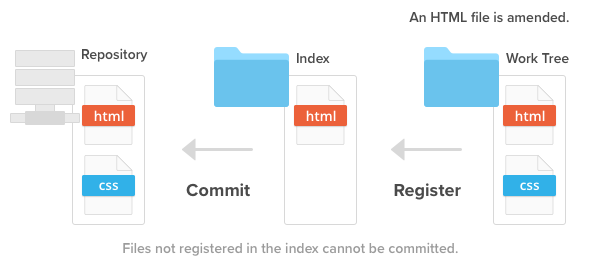
\includegraphics[scale=0.5]{images/git_workflow_001.png}
    \end{center}
    \caption{The three file states for Git: modified, staged, and committed.}
    \end{figure}

\chapter{Installing Git}
    \label{chap:installing}

    To install Git, please go to \href{https://git-scm.com/downloads}{https://git-scm.com/downloads} and download the version appropriate to your operating system.

    Alternatively, you can also install \href{https://windows.github.com}{GitHub for Windows} and have a nice GUI in addition to the CLI tools.

    Once installed, launch the git console or your OS's console (\verb|cmd| on Windows).
    There, run the following commands replacing \verb|<name>| by your name and \verb|<email>| by your email. These will be permanently attached to all commits you will make, so choose wisely.

    \begin{minted}[autogobble]{sh}
        git config --global user.name "<name>"
        git config --global user.email "<email>"
    \end{minted}

\chapter{Creating a repository}

    After installing Git on your machine as explained in chapter \ref{chap:installing}, the first thing you'll need to do is set up a repository. A repository (repo) is a centrally located folder for storing all your code. Once you create a Git repository with your files and directories, you can start tracking changes and versions. In this section, you'll learn how to get a repository up and running.

    \section{Remote repositories and local repositories}

    There are two types of Git repositories: remote and local.
    \begin{itemize}
        \item A remote repository is hosted on a remote, or off-site, server that is shared among multiple team members.
        \item A local repository is hosted on a local machine for an individual user.
    \end{itemize}

    While you can take advantage of Git version control features with a local repository, collaboration features—like pulling and pushing code changes with teammates—will be better suited on a remote repository.

    \begin{figure}[ht]
    \begin{center}
    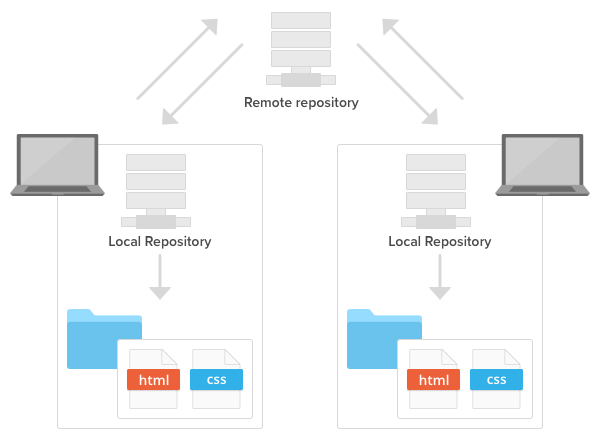
\includegraphics[scale=0.5]{images/creating_a_repository_001.png}
    \end{center}
    \caption{Git remote and local repositories working in harmony.}
    \end{figure}

    \section{How to create a repository}

    There are two ways to create a local repository on your machine. You can create a new repository from scratch using a file folder on your computer or clone an existing repository.

    \subsection{Git init}

    You can create a new repo from scratch using the \verb|git init| command. It can be used to introduce Git into an existing, unversioned project in order to start tracking changes.

    \subsection{Git clone}

    Use the \verb|git clone| command to copy a remote repository onto your local machine.

    By default, git clone automatically sets up a local master branch that tracks the remote master branch it was cloned from.

    A cloned repository has the same history log as the original one. You can refer and backtrack to any of those commits within your local repository.

    To clone a repository, run \verb|git clone <uri>| where \verb|<uri>| is the URI of the remote repository, on GitHub for example. It can be an http or ssh uri.

\chapter{Recording changes}

    Now that you understand how to create a git repository, you'll need to know how to save file changes.

    It is important to note that Git does not automatically save every change you make. You must tell Git which changes you want to be recorded by staging those changes. After staging, you can commit the changes so that they are recorded in the repo.

    \section{Making changes}

    As we mentioned in the Git workflow chapter (chapter \ref{chap:workflow}, changes are made in the working tree -- a directory consisting of the files you are currently working on. The working tree is where you edit files, add new files, and remove files that are no longer needed.

    All files that are changed in the working tree are noted as modified in the index. An index is a staging area where new commits are prepared. It sits between the repository and working tree.

    Changes made in the working tree will not be saved directly to the repository. All changes must first be staged in the index in order to be saved in the repo. Only the files in the index are committed to the repo.

    \section{Git commit}

    The git commit command enables you to record file changes in the repository's Git history.

    By committing, you will be able to view all changes chronologically in the respective file or directory.

    \begin{figure}[ht]
    \begin{center}
    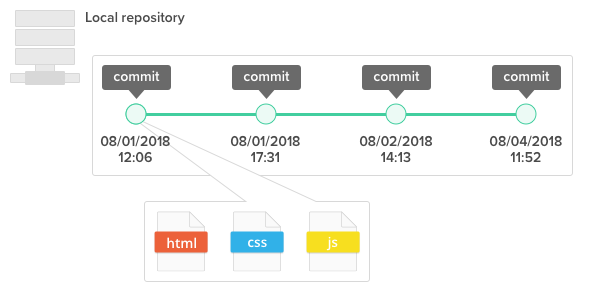
\includegraphics[scale=0.5]{images/recording_changes_001.png}
    \end{center}
    \caption{The commit history is stored in the local repository.}
    \end{figure}


    A 40-character checksum hash is used to uniquely identify a commit. You can use this checksum hash to retrieve the status or changes of files and directories that were made on the given commit in your repository.

    Separating different types of changes such as bug fixes, new features, and improvements into different sets of commits will allow you and your team members to easily understand why and how those changes were made.

    When committing your changes, you are required to enter a commit message. The commit message should provide descriptive comments regarding the changes you have made.

    Write commit messages that are descriptive and easy to understand for all your team members. The following is a recommended structure for an effective Git commit message:
    \begin{enumerate}
        \item 1st line: Abstract of the contents changed by commits
        \item 2nd line: Blank line
        \item 3rd line and the following lines: Reason for changes
    \end{enumerate}

    \subsection{Learn how to commit a file in Git.}

    Once you have edited a file, stage it using \verb|git add <filename>|.

    Then, once you have staged it, create the commit using \verb|git commit|. You will be asked for a commit message, fill it as indicated in the list above. Save and exit the temporary \verb|COMMITMSG| file to create the commit.

    If your repository is synced to a remote repository, run \verb|git push| to update the remote. Usage of that command is documented in section \ref{sec:push}.

\chapter{Syncing repositories}

    Remote repositories allow us to share our changes with other members of the team. They can be on a private server, on a different computer than yours, or hosted using a service like Backlog. Wherever yours is hosted, you'll need to be able to sync your local repository with the remote repository frequently. You'll do this using three commands: \verb|git push| (chapter \ref{chap:push-to-remote}), \verb|git pull| (chapter \ref{chap:pull-remote}), and \verb|git merge| (chapter \ref{chap:merge-branch}).

    \section{Git push}
    \label{sec:push}

    In order to start sharing changes with others, you have to push them to a remote repository using the \verb"push" command. This will cause the remote repository to update and synchronize with your local repository.

    \begin{figure}[ht]
    \begin{center}
    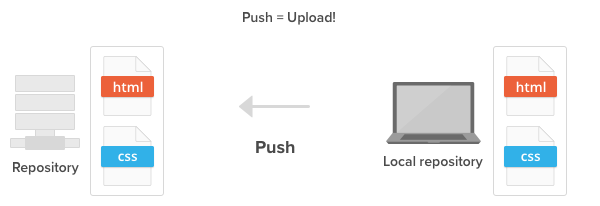
\includegraphics[scale=0.5]{images/syncing_repositories_001.png}
    \end{center}
    \caption{Push your local changes to a remote repository.}
    \end{figure}

    \section{Git pull}

    Whenever somebody pushes their changes to the shared remote repository, your local repository becomes out of date. To re-synchronize your local repository with the newly updated remote repository, simply run the \verb|git pull| operation.

    When the pull is executed, the latest revision history will download from the remote repository and import to your local repository.

    \begin{figure}[ht]
    \begin{center}
    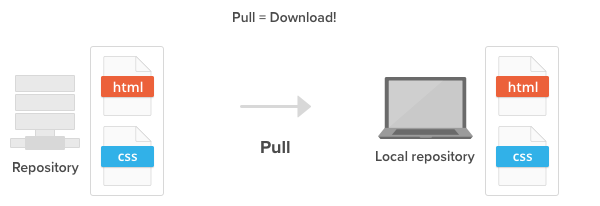
\includegraphics[scale=0.5]{images/syncing_repositories_002.png}
    \end{center}
    \caption{Pull changes from a remote repository to your local repository.}
    \end{figure}

    \chapter{Git merge}

    Your push to the remote repository will be rejected if your local repository is out of date, possibly because there are some updates on the remote repository that you do not have locally yet.

    \begin{figure}[ht]
    \begin{center}
    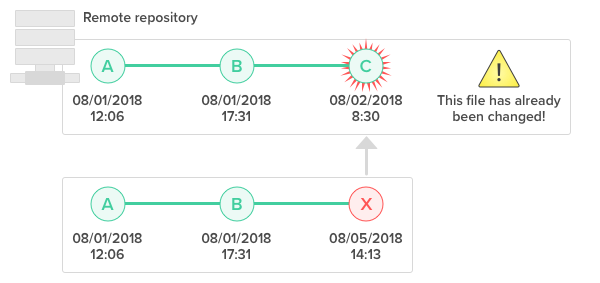
\includegraphics[scale=0.5]{images/syncing_repositories_003.png}
    \end{center}
    \caption{You are unable to push to the remote repository if your local repo is out of date.}
    \end{figure}

    If that is the case, you'll have to use the \verb|git merge| command to grab the latest change from the remote repository before you are allowed to push. Git enforces this to ensure that changes made by other members get retained in the history.

    \begin{figure}[ht]
    \begin{center}
    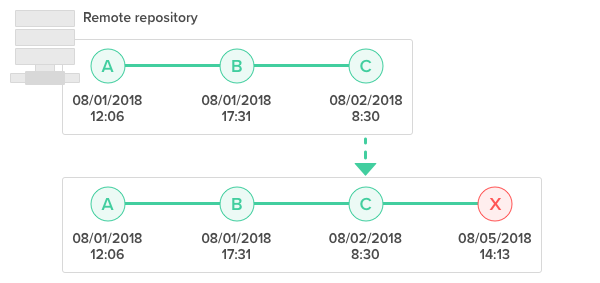
\includegraphics[scale=0.5]{images/syncing_repositories_004.png}
    \end{center}
    \caption{You must merge the latest changes before pushing.}
    \end{figure}

    During a \verb"merge", Git will attempt to automatically apply those history changes and merge them with the current branch. However, if there is a conflict in changes, Git will throw an error prompting you to resolve the conflict manually.

    \subsection{Resolve merge conflicts}

    When merging two branches, you may come across a conflict that needs resolving before you can properly complete the merge. For example, when two or more members make changes on the same part of a file in the two different branches (remote and local branches in this case), Git will not be able to automatically merge them.

    When this happens, Git will add some standard conflict-resolution markers to the conflicting file. The markers help you figure out which sections of the file need to be manually resolved.

    \begin{figure}[ht]
    \begin{center}
    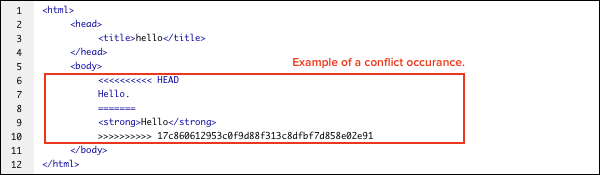
\includegraphics[scale=0.5]{images/syncing_repositories_005.png}
    \end{center}
    \caption{Example of a conflict occurrence.}
    \end{figure}

    In our example, everything above \verb"=====" is your local content, and everything below it comes from the remote branch.

    You must resolve the conflicting parts as shown below before you can proceed with creating a merge commit.

    \begin{figure}[ht]
    \begin{center}
    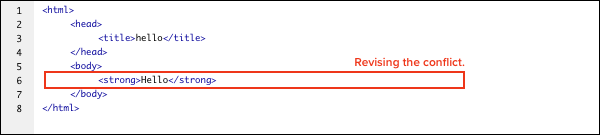
\includegraphics[scale=0.5]{images/syncing_repositories_006.png}
    \end{center}
    \caption{Revise the commit to eliminate the conflict.}
    \end{figure}

\part{Collaboration}

\chapter{Using branches}

    In a collaborative environment, it is common for several developers to share and work on the same source code. While some developers will be fixing bugs, others will be implementing new features, etc. With so much going on, there needs to be a system in place for managing different versions of the same code base.

    Branching allows each developer to branch out from the original code base and isolate their work from others. It also helps Git to easily merge versions later on.

    \section{What is a Git branch?}

    A Git branch is essentially an independent line of development. You can take advantage of branching when working on new features or bug fixes because it isolates your work from that of other team members.

    \begin{figure}[ht]
    \begin{center}
    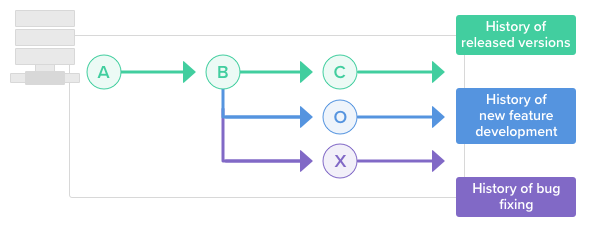
\includegraphics[scale=0.5]{images/using_branches_001.png}
    \end{center}
    \caption{A git branch is an independent line of development taken from the same source code.}
    \end{figure}

    Different branches can be merged into any one branch as long as they belong to the same repository.

    Diagram \ref{fig:parallel-using-branches} illustrates how development can take place in parallel using branches.

    \begin{figure}[ht]
    \begin{center}
    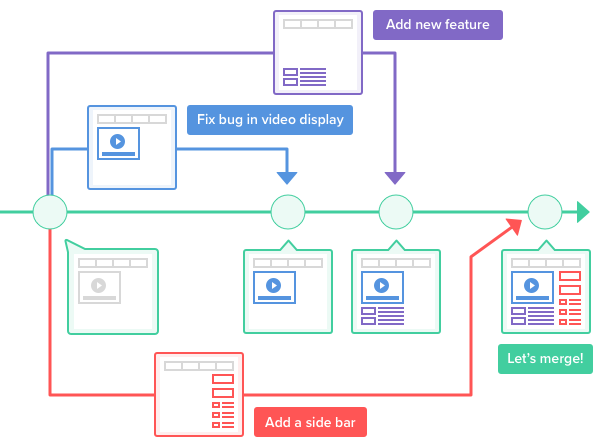
\includegraphics[scale=0.5]{images/using_branches_002.png}
    \end{center}
    \caption{Multiple development projects taking place using the same source code.}
    \label{fig:parallel-using-branches}
    \end{figure}

    Branching enables you to isolate your work from others. Changes in the primary branch or other branches will not affect your branch, unless you decide to pull the latest changes from those branches.

    It is a common practice to create a new branch for each task (i.e., a branch for bug fixing, a branch for new features, etc.). This method allows others to easily identify what changes to expect and also makes backtracking simple.

    \section{Create a branch}

    Creating a new branch does not change the repository; it simply points out the commit

    For example, let's create a branch called “issue1” using the command git branch.
    \begin{minted}[autogobble]{sh}
    git branch issue1
    \end{minted}

    Illustration \ref{fig:new-branch} provides a visual on what happens when the branch is created. The repository is the same, but a new pointer is added to the current commit.

    \begin{figure}[ht]
    \begin{center}
    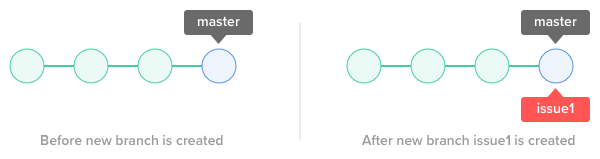
\includegraphics[scale=0.5]{images/using_branches_003.png}
    \end{center}
    \caption{Before new branch is created}
    \label{fig:new-branch}
    \end{figure}

\chapter{Switch branches}

    The \verb|git checkout| command allows you to switch branches by updating the files in your working tree to match the version stored in the branch that you wish to switch to.

    You can think of it as a way of switching between different workspaces.

    \section{Git HEAD}

    \verb|HEAD| is used to represent the current snapshot of a branch. For a new repository, Git will by default point \verb|HEAD| to the master branch. Changing where \verb|HEAD| is pointing will update your current active branch.

    The \verb|~|(tilde) and \verb|^|(caret) symbols are used to point to a position relative to a specific commit. The symbols are used together with a commit reference, typically \verb|HEAD| or a commit hash.

    \verb|~<n>| refers to the <n>th grandparent. \verb|HEAD~1| refers to the commit's first parent. \verb|HEAD~2| refers to the first parent of the commit's first parent.

    \verb|^<n>| refers to the the <n>th parent. \verb|HEAD^1| refers to the commit's first parent. \verb|HEAD^2| refers to the commit's second parent. A commit can have two parents in a merge commit.
    \verb|~|(tilde) and \verb|^|(caret) symbols point to a position relative to the commit
    \verb|~|(tilde) and \verb|^|(caret) symbols point to a position relative to the commit

    \section{Git Stash}

    Whenever you switch to another branch with uncommitted changes (or new files added) in your working tree, these uncommitted changes will also be carried to the new branch that you switch to. Changes that you commit will be committed to the newly switched branch.

    However, if Git finds a conflict between the files from the newly switched branch and the uncommitted changes from the previous branch, you will not be allowed to switch to the other branch. You must commit or stash those changes first before switching branches.

    You can think of stash as a drawer to store uncommitted changes temporarily. Stashing allows you to put aside the “dirty” changes in your working tree and continue working on other things in a different branch on a clean slate.

    Uncommitted changes that are stored in the stash can be taken out and applied to the original branch and other branches as well.

    To stash changes, just run \verb|git stash|. To take out changes from the stash, run \verb|git stash pop|.

\chapter{Remote branches}

    Although Git is local on your computer, you can also have remote copies of a repository. Remote repositories can be on a private central server or even simply on a coworker's computer.

    You can also have a remote repository hosted using an online service–such as Backlog.

    You can retrieve others' changes to the repository or move your local copy of a repository to the remote server.

\chapter{Pull remote branch}
    \label{chap:pull-remote}

    You can apply the latest changes from a remote repository to your local repository using the \verb|git pull| command.

    For example, say the remote branch is upstream of your local branch. The remote branch would include all of the changes that belong to the local branch as shown below.

    \begin{figure}[ht]
    \begin{center}
    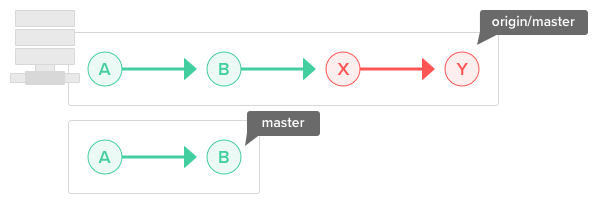
\includegraphics[scale=0.5]{images/pull_remote_branch_001.png}
    \end{center}
    \caption{Remote branch is upstream from local branch.}
    \end{figure}

    In this case, if we were to apply a merge from the remote branch (origin/master) into our local branch (master), it would be a fast-forward merge.

    \begin{figure}[ht]
    \begin{center}
    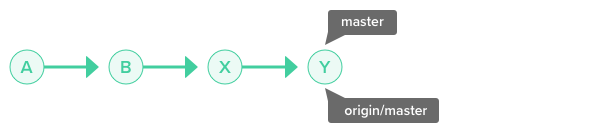
\includegraphics[scale=0.5]{images/pull_remote_branch_002.png}
    \end{center}
    \caption{Fast-forward merge}
    \end{figure}

    However, if there are changes in the local master branch that are not present in the remote origin/master branch, the \verb|git pull| command will execute a merge and create a merge commit that ties those changes together. If you don't want the upstream changes to be merged automatically, see \verb|git fetch|, chapter \ref{chap:fetch-remote}.

    \begin{figure}[ht]
    \begin{center}
    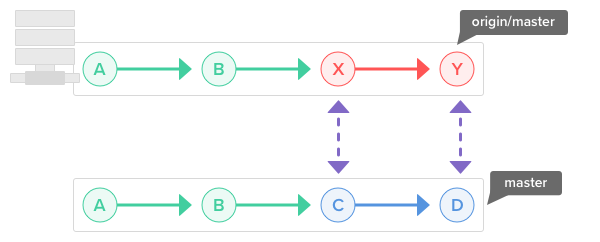
\includegraphics[scale=0.5]{images/pull_remote_branch_003.png}
    \end{center}
    \caption{Git must merge and commit before a pull if the local branch is different from the remote branch.}
    \end{figure}

    When a pull is executed, a merge commit will be automatically created in the local repository. If there is a conflict, you will have to resolve the conflict and commit the merge manually.

    \begin{figure}[ht]
    \begin{center}
    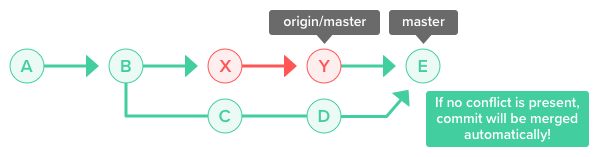
\includegraphics[scale=0.5]{images/pull_remote_branch_004.png}
    \end{center}
    \caption{If there is no conflict, the commit will be merged automatically.}
    \end{figure}

\chapter{Fetch remote branch}
    \label{chap:fetch-remote}

    When you execute a pull, the changes from the remote branch automatically merge into your current local branch. If you want to obtain the remote changes but not have them merged into your current local branch, you can execute the \verb|git fetch| command.

    Fetch will download the changes from remote that do not yet exist on your local branch. The \verb|FETCH_HEAD| ref can be used to track the fetched changes from the remote repository.

    The revision history will look like in figure \ref{fig:fetch-remote-001} when both the remote and local branch contain different descendants.

    \begin{figure}[ht]
    \begin{center}
    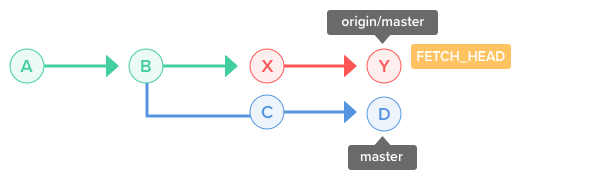
\includegraphics[scale=0.5]{images/fetch_remote_branch_001.png}
    \end{center}
    \caption{Revision history when remote and local branches have different masters}
    \label{fig:fetch-remote-001}
    \end{figure}

    Once changes are fetched, you can apply those changes to your local repository by merging in \verb|FETCH_HEAD| or by executing a pull.

    \begin{figure}[ht]
    \begin{center}
    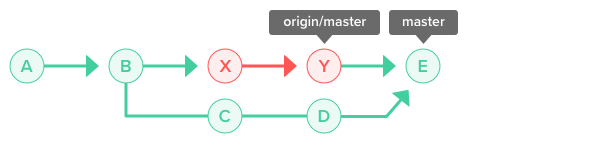
\includegraphics[scale=0.5]{images/fetch_remote_branch_002.png}
    \end{center}
    \caption{After merging, changes will be applied to the local repo}
    \end{figure}

    Once \verb|FETCH_HEAD| has been merged, the revision history will yield the same result as a git pull operation. Pull is essentially a simultaneous execution of fetch and merge operations.

\chapter{Push branch to remote}
    \label{chap:push-to-remote}

    All of your commits are available to you until you push your local branch to the remote repository. That is, you can work on your own local branch at your own pace without affecting other members of the team.

    When you push your local branch to remote, Git will do a fast-forward merge to the destination repository.

    However, if the push results in a non-fast-forward merge, Git will decline your push to prevent you from overwriting previous commits. In that case, you have to pull the latest remote changes and push again.

    \begin{figure}[ht]
    \begin{center}
    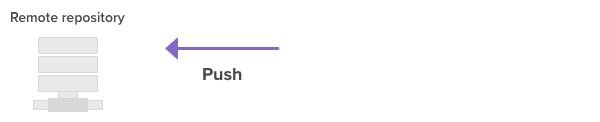
\includegraphics[scale=0.5]{images/push_branch_to_remote_001.png}
    \end{center}
    \caption{Use git push to add your local changes to the remote repository}
    \end{figure}

    You must not overwrite or change commits that have already been committed to the remote repository. Doing so will cause other team members' local repositories to desynchronize with the remote repository. \emph{When you want to run} \verb|git push --force|\emph{, run }\verb|git push --force-with-lease|\emph{ instead.} It won't allow you to overwrite changes that you don't have in your local repository, thus new commits won't be lost.

\chapter{Branching workflows}

    Let's take a look at the Gitflow Workflow as outlined in A successful Git branching model.

    This workflow consists of five types of branches, each with different roles:
    \begin{itemize}
        \item Master (\ref{sec:branching:master})
        \item Feature branch (aka Topic branch) (\ref{sec:branching:feature-branch})
        \item Release branch (\ref{sec:branching:release-branch})
        \item Hotfix branch (\ref{sec:branching:hotfix-branch})
        \item Develop branch (aka Integration branch) (\ref{sec:branching:develop-branch})
    \end{itemize}

    \emph{At the BDI, we typically only use master and develop branches, although you are encouraged to create feature branches to work.}

    \begin{figure}[ht]
    \begin{center}
    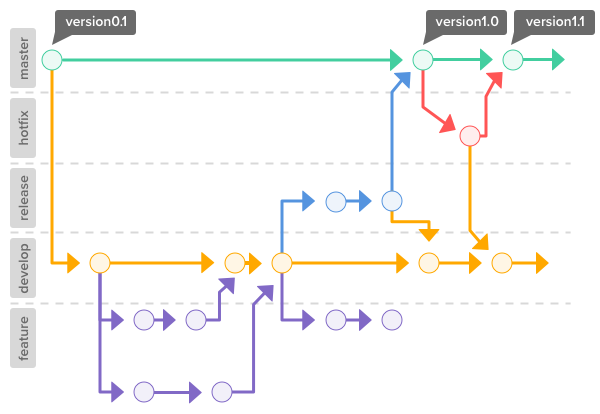
\includegraphics[scale=0.5]{images/branching_workflows_001.png}
    \end{center}
    \caption{Basic Git branching workflow with master, topic, release, and hotfix branches}
    \end{figure}

    \section{Master}
    \label{sec:branching:master}

    Upon making the first commit in a repository, Git will automatically create a master branch by default. Subsequent commits will go under the master branch until you decide to create and switch over to another branch.

    Codebase residing in the master branch is considered to be production-ready. When it is ready for a specific release, the latest commit will be given a \emph{release tag}.

    \begin{figure}[ht]
    \begin{center}
    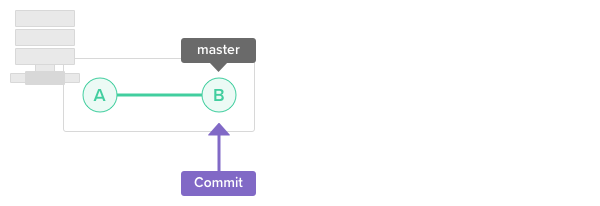
\includegraphics[scale=0.5]{images/branching_workflows_002.png}
    \end{center}
    \caption{Changes are committed to the master branch}
    \end{figure}

    \section{Feature/Topic branch}
    \label{sec:branching:feature-branch}

    When you start working on a new feature/bug fix, you should create a feature/topic branch. A feature/topic branch is normally created off a develop/integration branch. This feature/topic branch can reside in your local machine throughout the entire development lifecycle of the feature.

    You will push this branch to the remote repository whenever you are ready to merge the change set with the develop/integration branch.

    \begin{figure}[ht]
    \begin{center}
    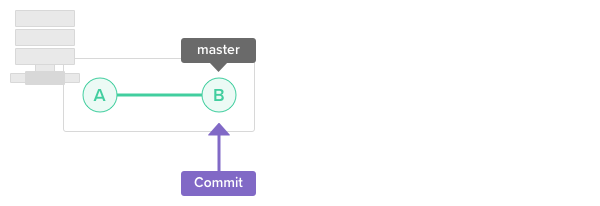
\includegraphics[scale=0.5]{images/branching_workflows_002.png}
    \end{center}
    \caption{Feature branches}
    \end{figure}

    \section{Release branch}
    \label{sec:branching:release-branch}

    When you roll out a new release, you create a release branch. A release branch helps you to ensure that the new features are running correctly.

    By convention, release branch names normally start with the prefix \verb"release-".

    The release branch is typically created off the develop/integration branch when it's close to being production-ready.

    Only bug fixes and release related issues should be addressed on this branch. Having this branch will allow other team members to continue pushing new features to the develop/integration branch without interrupting the release workflow.

    When you are ready to release, merge the release branch with the master branch and tag a release number to the newly created merge commit.

    You should also merge the release branch with the develop/integration branch so that both the master and develop/integration branches receive the latest changes/bug fixes from the release branch.

    \section{Hotfix branch}
    \label{sec:branching:hotfix-branch}

    When you need to add an important fix to your production codebase quickly, you can create a Hotfix branch off the master branch.

    By convention, hotfix branch names normally start with the prefix "hotfix-".

    The advantage of a hotfix branch is that it allows you to quickly issue a patch and have the change merged with the master branch without having to wait for the next release.

    A hotfix branch should be merged with the develop/integration branch as well.

    \section{Develop/Integration branch}
    \label{sec:branching:develop-branch}

    A develop/integration branch should be kept stable at all times. This is important because new branches are created off of this branch, and this branch could eventually go out live on production. Continuous integration tools such as Jenkins can be used to help do just that.

    When some changes need to be merged into the develop/integration branch, it is generally a good idea to create a feature/topic branch to work on independently.

\chapter{Integrating branches}
    \label{chap:integrating-branches}

    Once you are done working on a feature/topic branch (i.e., new feature or bug fix), you would typically merge it with a develop/integration branch. You can accomplish that by using the git merge or git rebase commands, although both commands will give you different results.

    \begin{description}
        \item[Merge] Retains all changes to and history of the merged branch. The revision history can become complicated after many merge commits.

        \item[Rebase] Maintains a clean revision history since merged commits are appended at the end of the target branch. Conflicts may occur more often than in the merge method, and they need to be resolved immediately.
    \end{description}

    You and your team should decide on which method of merging to use. If you want to keep your revision history simple, you can do the following :
    \begin{itemize}
        \item Use rebase on your feature/topic branch when you want to pull the latest change from the develop/ integration branch.
        \item If you want to merge the change from your feature/topic branch to the develop/integration branch, rebase the feature/topic branch onto the develop/integration branch first. After which, merge the changes from the feature/topic branch into the develop/integration branch. This will be a fast-forward merge with no extra merge commits being created.
    \end{itemize}

    At the BDI, we have chosen to always merge using GitHub Pull Requests. Once your feature branch is ready, create a pull request on the repository pull requests page with base \verb|develop| and compare \verb|<feature-branch>|. See chapter \ref{chap:pull-requests} for more about them.

\chapter{Merge branch}
    \label{chap:merge-branch}

    You can integrate several branches by using the git merge command.

    Consider the situation in figure \ref{fig:bugfix-ff-possible}. There are two branches: a "bugfix" branch with a few commits coming off the "master" branch.

    \begin{figure}[ht]
    \begin{center}
    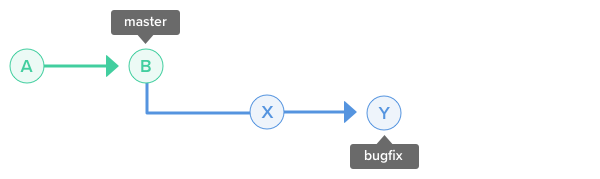
\includegraphics[scale=0.5]{images/merge_branch_001.png}
    \end{center}
    \caption{A fast-forward is possible from master to bugfix}
    \label{fig:bugfix-ff-possible}
    \end{figure}

    In this case, merging "bugfix" back into "master" is not much of an issue. That's because the state of "master" has not changed since "bugfix" was created. Git will merge this by moving the "master" position to the latest position of "bugfix". This merge is called a "fast-forward".

    \begin{figure}[ht]
    \begin{center}
    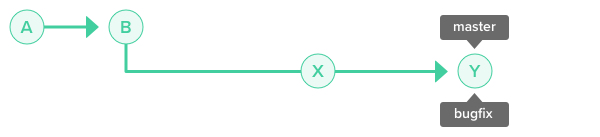
\includegraphics[scale=0.5]{images/merge_branch_002.png}
    \end{center}
    \caption{Fast-forward merge}
    \end{figure}

    In the example in figure \ref{fig:master-advance-bugfix}, however, "master" has been updated several times since "bugfix" was branched out. The changes from "bugfix" and "master" need to be combined when a merge is executed on these two branches.

    \begin{figure}[ht]
    \begin{center}
    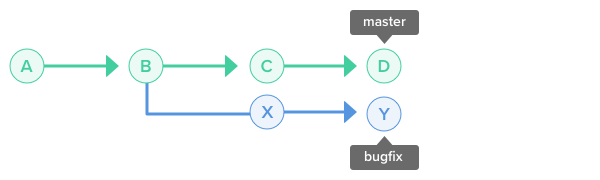
\includegraphics[scale=0.5]{images/merge_branch_003.png}
    \end{center}
    \caption{master has new commits since bugfix's creation}
    \label{fig:master-advance-bugfix}
    \end{figure}

    For this sort of merge, a "merge commit" will be created and the "master" position will be updated to the newly created merge commit.

    \begin{figure}[ht]
    \begin{center}
    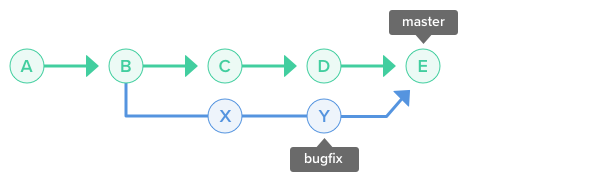
\includegraphics[scale=0.5]{images/merge_branch_004.png}
    \end{center}
    \caption{Merge commit incorporating both changes}
    \end{figure}

    Even when a fast-forward merge is possible, you could still explicitly force it to merge without a fast-forward merge. Use \verb|git merge --no-ff <branch>| for that.

    \begin{figure}[ht]
    \begin{center}
    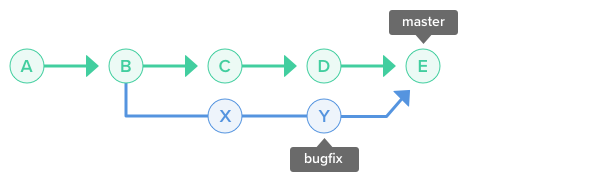
\includegraphics[scale=0.5]{images/merge_branch_004.png}
    \end{center}
    \caption{Non fast-forward merge}
    \label{fig:no-ff-merge}
    \end{figure}

    As shown in figure \ref{fig:no-ff-merge}, a non fast-forward merge leaves the "bugfix" branch as it is. This leaves you with a clearer picture of the feature/topic branch "bugfix". You can easily find where the feature/topic branch starts or ends and also track the changes that are made to the feature/topic branch.

    At BDI, we ask you to always use non fast-forward merges because it makes it easier to see how the history changed, and who merged branches. Also, prefer pull requests over merging manually. For more about pull-requests, see chapter \ref{chap:pull-requests}.

\chapter{Rebase branch}

    For a cleaner revision history, you can use the \verb|git rebase| command to integrate your branches. \emph{We do not use it at BDI!}

    Say we have two branches with a non fast-forward merge scenario as shown in figure \ref{fig:non-ff-scenario}.

    \begin{figure}[ht]
    \begin{center}
    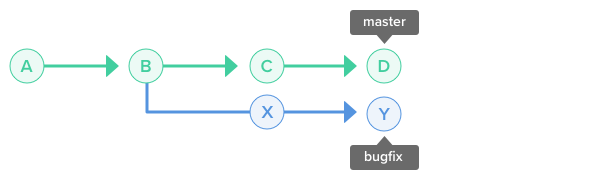
\includegraphics[scale=0.5]{images/rebase_branch_001.png}
    \end{center}
    \caption{Two branches with a non fast-forward merge scenario}
    \label{fig:non-ff-scenario}
    \end{figure}

    Doing a rebase will result in the branch history looking similar to the example in figure \ref{fig:unify-branches}.

    \begin{figure}[ht]
    \begin{center}
    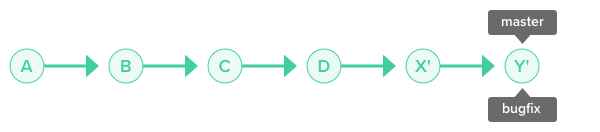
\includegraphics[scale=0.5]{images/rebase_branch_002.png}
    \end{center}
    \caption{Unify branches by using rebase}
    \label{fig:unify-branches}
    \end{figure}

    When you rebase a bugfix branch to the master branch, commits from the bugfix branch will be replayed and appended to the end of the master branch. The end result is a single simple stream of commits in the bugfix branch history.

    In the event of a conflict when the commit is being appended, you will be asked by Git to fix the conflict before proceeding with rebasing the other commits.

    \begin{figure}[ht]
    \begin{center}
    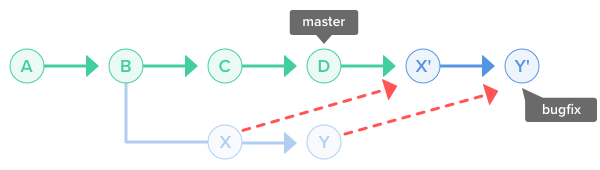
\includegraphics[scale=0.5]{images/rebase_branch_003.png}
    \end{center}
    \caption{Unify branches by using rebase with conflicts}
    \end{figure}

    A rebase does not move the position of the master. In any case, you will be able to do a fast-forward or a clean merge from bugfix to master after rebasing.

    \begin{figure}[ht]
    \begin{center}
    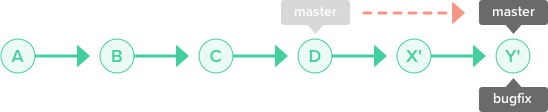
\includegraphics[scale=0.5]{images/rebase_branch_004.png}
    \end{center}
    \caption{Fast-forward merge after a rebase}
    \end{figure}

\chapter{Tags}

    A Git tag is used to label and mark a specific commit in the history. Tags are commonly used to indicate release versions, with the release name (i.e., v1.0) being the name of the tag.

    There are two types of Git tags:
    \begin{itemize}
        \item Lightweight tag
        \item Annotated tag
    \end{itemize}

    A lightweight tag is similar to a branch that does not change. It just points directly to a specific commit in the history. Lightweight tags are mainly used temporarily in your local workspace.

    An annotated tag is checksummed and often used when you are planning to mark an important commit. You can add comments, a signature, the date, plus the tagger's name and e-mail.

\chapter{Pull requests}
    \label{chap:pull-requests}

    There are many questions and opinions when it comes to reviewing source code. Code review can be difficult to stick with because people become busy with other tasks or feel it is too time consuming to go through the changes that have been made. Often, code review becomes a neglected task.

    It can be challenging to make code review an integral part of your team's workflow; pull requests make that easier.

    \begin{figure}[ht]
    \begin{center}
    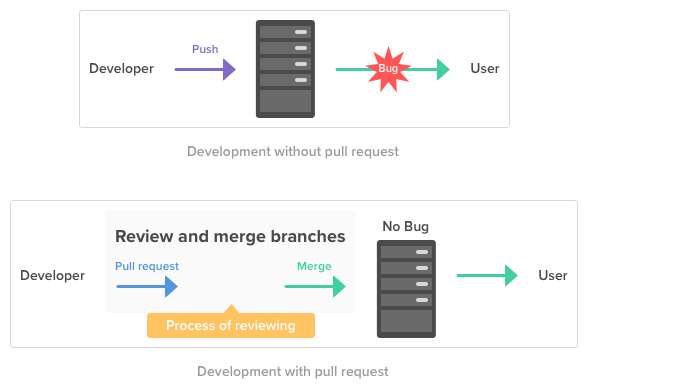
\includegraphics[scale=0.5]{images/pull_requests_001.png}
    \end{center}
    \caption{Development without or with pull requests}
    \end{figure}

    A pull request notifies other development team members of changes made in your local repository. Pull requests provide the following functions:
    \begin{itemize}
        \item Notify team members when a review or merge of work is needed
        \item Display changes made to source code in an easy-to-understand manner
        \item Provide a platform for communicating about source code
    \end{itemize}

    Pull requests are not a Git function. They were created by GitHub to make it easier for developers to participate in open source development, and, as a result, enabled them to create higher-quality source code. Pull requests are available in most major Git hosting services, such as Backlog, GitLab and Bitbucket.

    \section{Benefits of pull requests}

    In figure \ref{fig:pr-list} are a list of pull requests in GitHub. You can easily see which ones are open or have not been completed. This makes it easy for team members to review pull requests.

    \begin{figure}[ht]
    \begin{center}
    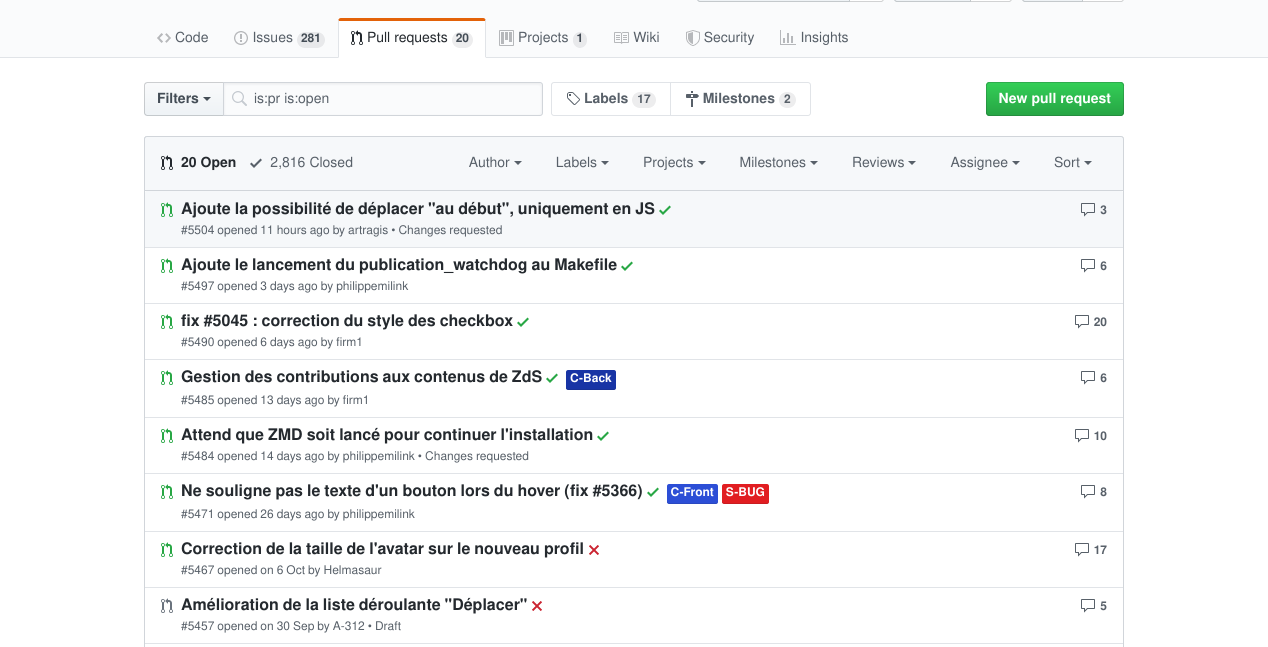
\includegraphics[scale=0.35]{images/pull_requests_002.png}
    \end{center}
    \caption{Pull request list in GitHub, a Git hosting service with bug tracking features.}
    \label{fig:pr-list}
    \end{figure}

    The creator and reviewer of a pull request can have discussions right on the page using comments. These comments are recorded on the server, so they can be revisited at a later time.g

    You can also commit and push changes to a specific branch. The pushed commit will automatically be reflected in the pull request.

    This structured code review leads to higher quality source code and provides greater context for future discussions.

    \begin{figure}[htp]
    \begin{center}
    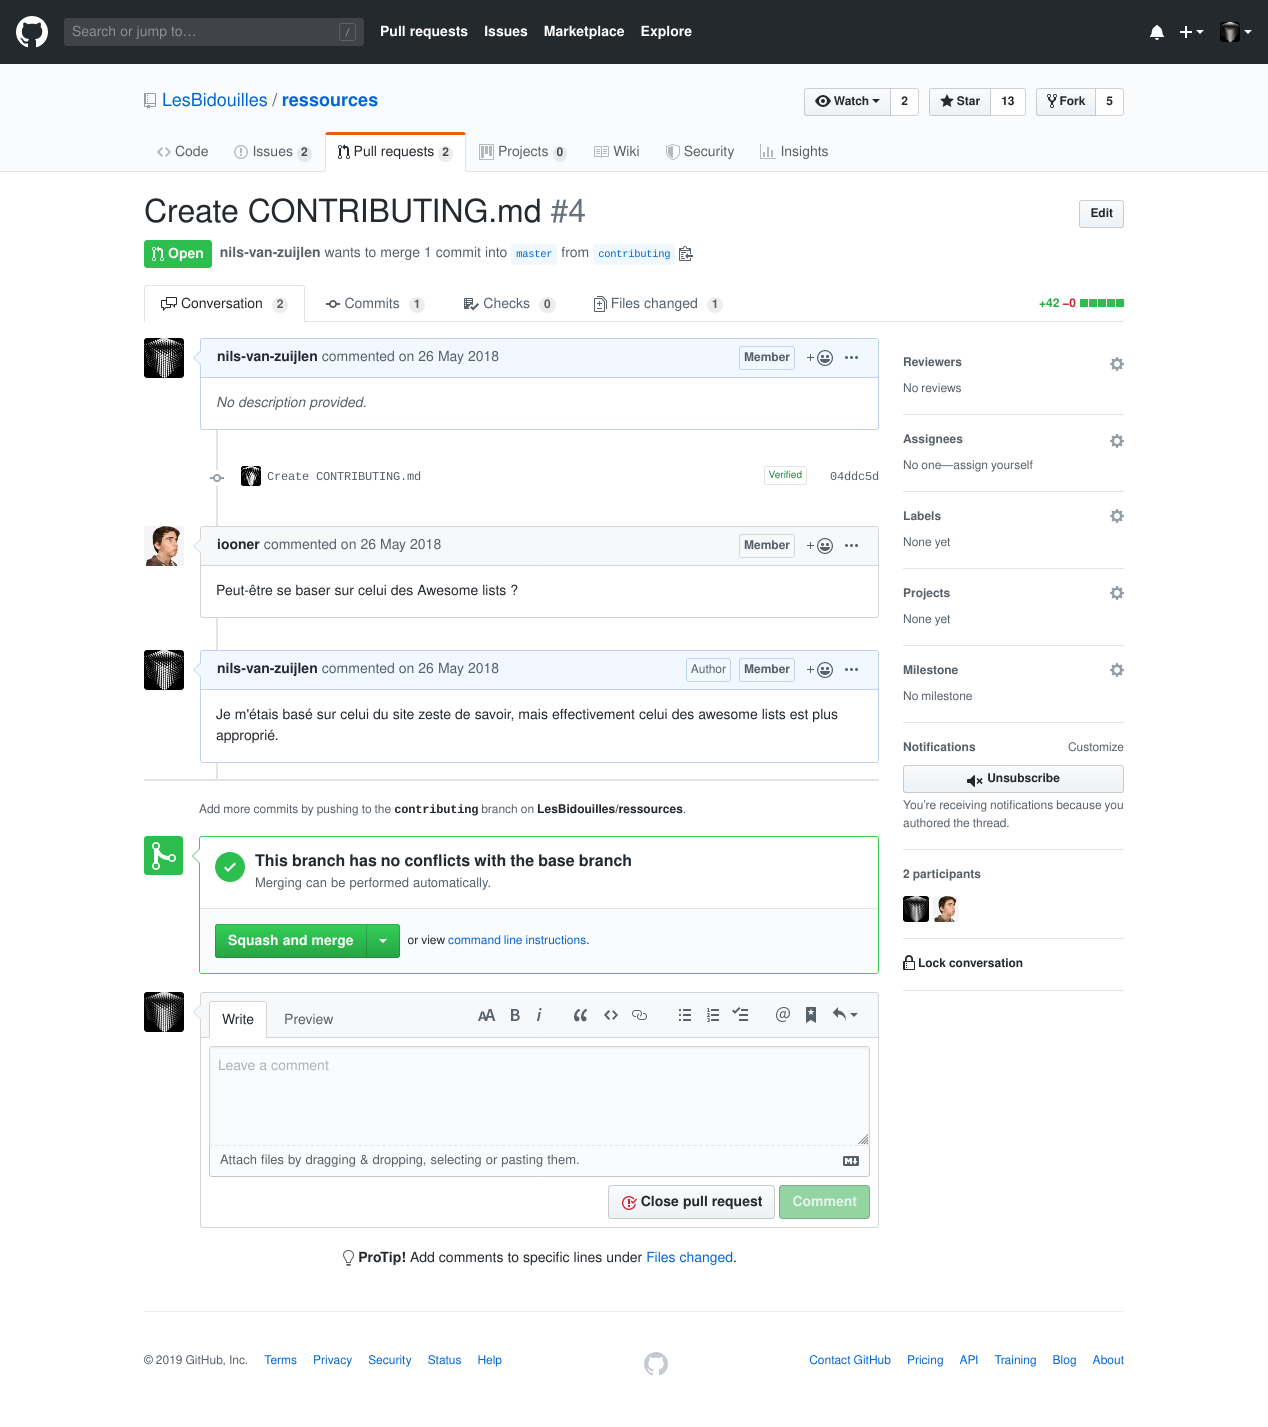
\includegraphics[scale=0.3]{images/pull_requests_003.png}
    \end{center}
    \caption{Pull request comments in GitHub.}
    \end{figure}

    Pull request clearly display what changes have been made to source code. The pull request creator can also add notes about what their goal was for the source code and provide supplementary information. This info helps inform the reviewer.

    \begin{figure}[ht]
    \begin{center}
    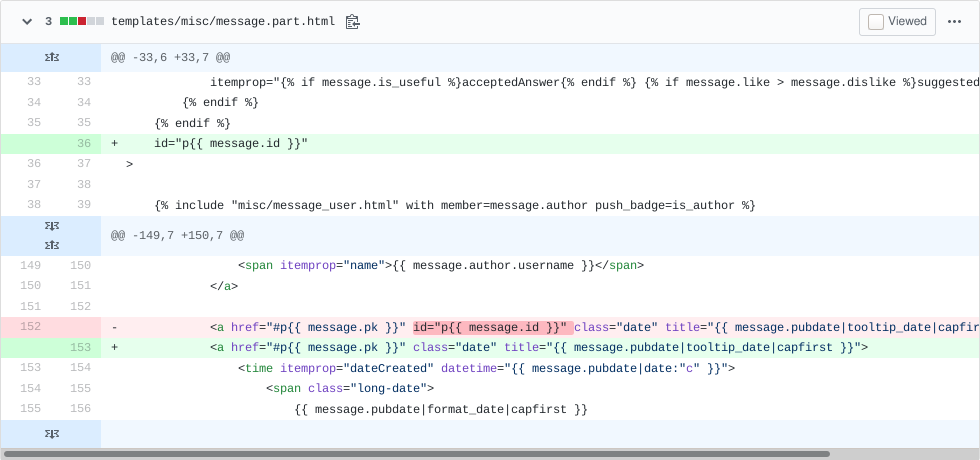
\includegraphics[scale=0.45]{images/pull_requests_004.png}
    \end{center}
    \caption{Changes are highlighted in the source code.}
    \end{figure}

    \section{Development process with pull requests}

    Here is a simple development workflow with pull requests your team can follow:
    \begin{enumerate}
        \item [Developer] Clone or pull the source of the work target.
        \item [Developer] Create a branch for the work.
        \item [Developer] Perform development work such as adding and modifying functions.
        \item [Developer] Push after the task is completed.
        \item [Developer] Create a pull request.
        \item [Review / Merge Personnel] Check the changes from the notified pull request and review.
        \item [Review / Merge Personnel] Judge the work and send a feedback to the developer if necessary.
        \item [Review / Merge Personnel] Merge if there is no problem as a result of the review.
        \item [Review / Merge Personnel] Close if the pull request itself becomes unnecessary as a result of the review.
    \end{enumerate}

    Repeat steps 3 through 7 as often as needed to improve the quality of the source code.

    \begin{figure}[ht]
    \begin{center}
    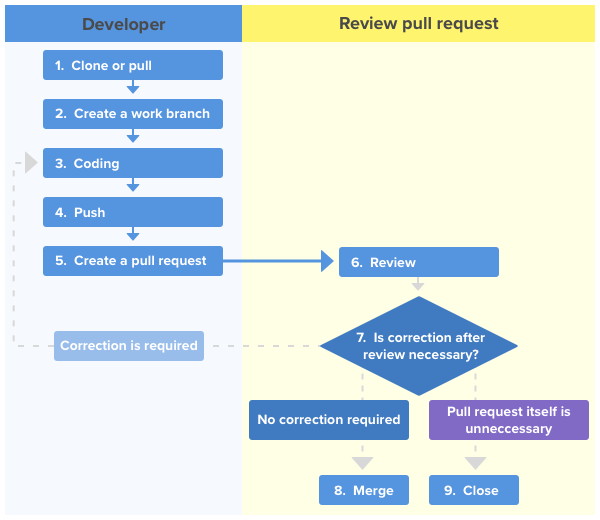
\includegraphics[scale=0.5]{images/pull_requests_005.png}
    \end{center}
    \caption{Development process with pull requests}
    \end{figure}

\end{document}
